% --------------------------------------------------------------
% This is all preamble stuff that you don't have to worry about.
% Head down to where it says "Start here"
% --------------------------------------------------------------

\documentclass[12pt]{article}

\usepackage[margin=1in]{geometry}
\usepackage{setspace,fancyhdr,listings,xcolor,graphicx,adjustbox}

\usepackage[colorlinks=true, linkcolor=blue, urlcolor=blue]{hyperref} % Configures hyperlink color

\lstset{
    language=C,
    numbers=left,
    numberstyle=\tiny\color{gray},
    stepnumber=1,
    numbersep=10pt,
    backgroundcolor=\color{white},
    showspaces=false,
    showstringspaces=false,
    showtabs=false,
    frame=single,
    rulecolor=\color{black},
    tabsize=2,
    captionpos=b,
    breaklines=true,
    breakatwhitespace=false,
    title=\lstname,
    keywordstyle=\color{blue},
    commentstyle=\color{green},
    stringstyle=\color{red},
    basicstyle=\ttfamily\footnotesize,
    escapeinside={\%*}{*)},
    morekeywords={*,...},
    lineskip=-1pt % Adjust this value to make lines more compact
}
\pagestyle{fancy}
\fancyhf{}

\setlength{\headheight}{15pt}
\fancyhead[R]{Topete \thepage}

\begin{document}

% --------------------------------------------------------------
%                         Start here
% --------------------------------------------------------------

\title{EE/CS 120B Custom Laboratory Project Report\\
Guess The Color}
\author{Danny Topete}

\maketitle

\doublespacing

\section{Introduction:}
I wrote a guess the color game. The idea originally came from watching a friend 
be good at CSSbattle.net,
I always aspired to be that good at him at guessing the hex values instantly and rebuilding a website like that.
So I decided to make a game that would help me practice!

In terms of the UI, there is a main menu that gives you a play button. After you press play,
a random color is presented to, a prompt to enter the
hex code of the presented color. Then a percentage
of how close you are to the target value. Along with
a timer that records how fast you solve it.
As you solve the colors, the Shift Register turns on one of the
three LEDs on the small board.

\href{https://youtu.be/q6jeuhIvPzk}{Final Project Demo Video}

\pagebreak
\section{Build Upons:}
\begin{enumerate}
  \item \textbf{ST7735 Display:}
    There are two scenes, the start menu, and the playing scene.
    The start menu's functionality is to show the in the center "PLAY"
    (which is doing a chroma animation),
    and, after you press any input, it goes straight into the game.
    This main menu plays a huge role. It serves to keep rolling rand()
    in the background which almost simulates having
    a unique srand() seed after every single boot.

    Then, there is the play scene. This is where you have the RGB LED
    display a random color, and you have to guess the hex value.
  \item \textbf{Shift Register - 74HC595:} This was implemented successfully.
    The only issue is that I believe there are insulation issues, hence why they flicker.

    When ever I touch the cables, the three LEDs turn off.
    I notice that when I unplug the VCC, the lights are stable and don't flicker.
    But this only works while the RED LED is on. 


    I believe this is either poor insulation, or the arduino
    just doesn't have enough power. 
    This may be a hardware limitation to where it does not want to be one while 
    other things are being computed. Or just the fact that 5V is very limited for this circuit.
    It does not take away from the functionality.
  \item \textbf{IR Sensor / NEC Remote:}
    The IR tasks and sensor works perfectly,
    I have minimized the amount of times it returns trash values, by setting a higher
    period. Besides that, sometimes the IR sensor doesn't read if the display is being updated,
    and again, I believe this is more hardware limitations of the microcontroller.
\end{enumerate}

\pagebreak
\section{User Guide:}
\begin{itemize}
  \item When you begin in the start screen, you will be presented with a
    simple prompt. To get out of the prompt and play the game, just press any button.
    You may need to hold down any button until you get the play scene.
  \item In the play scene, you will be presented with an RGB LED being lit up
    to a random color and a hex value that you input.
    \item\subsection*{Game's Inputs:}
\begin{minipage}{0.7\textwidth}
    \begin{itemize}
        \item \textbf{Power Button:} This will roll you a new color.
        \item \textbf{1:} This will iterate your red hex value.
        \item \textbf{4:} This will lower your hex value by one.
        \item \textbf{2:} This will iterate your green hex value.
        \item \textbf{5:} This will lower your green hex value by one.
        \item \textbf{3:} This will iterate your blue hex value.
        \item \textbf{6:} This will lower your blue hex value by one.
    \end{itemize}
\end{minipage}%
\hfill
\begin{minipage}{0.28\textwidth}
    \centering
    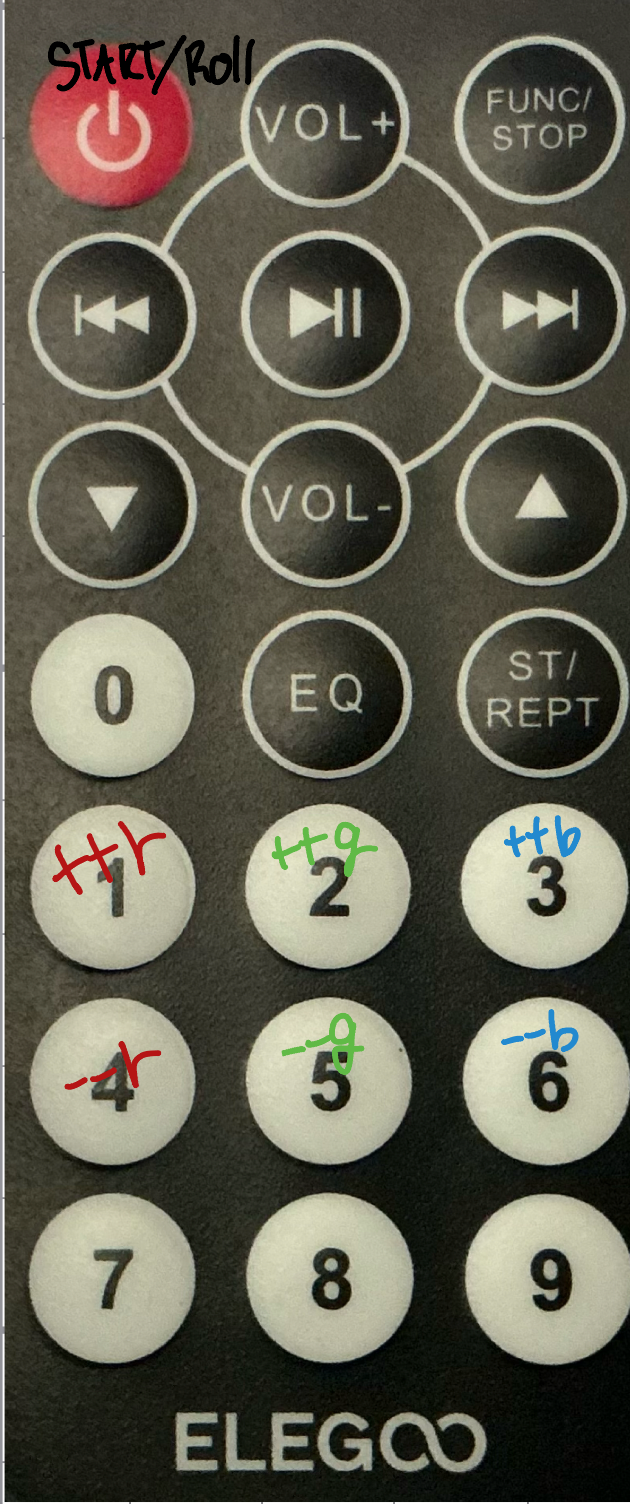
\includegraphics[width=\textwidth]{remote.png}
    % Add arrows or labels using external tools or include the annotated image.
\end{minipage}

\pagebreak
  \item You will need to guess the color that the RGB-LED is displaying.
  \item As you get the closer to the color, the lights in the little board
    that are connected to the shift register will start outputting values.
    \begin{itemize}
      \item Example: If you get the value of red correctly,
        the shift register turn on the Red LED.
        Along with the display putting a box over the hex value you have correctly guessed.
    \end{itemize}
  \item After you have correctly guessed the color, you will be greeted with your
    elapsed time being paused and showing in chroma mode.
    This means you have won, and pressing
    the power button will put you into the main menu to start again.
\end{itemize}

\pagebreak
\section{Hardware:}
\begin{enumerate}
  \item \textbf{ST7735 Display:}
    Successfully implemented
  \item \textbf{RGB LED:}
    This one was successfully implemented, except for the part
    where it flickers a bit while the display is updating.
    I believe this is power issues. But it doesn't take away
    from the functionality.
  \item \textbf{Shift Register:} This was implemented successfully.
  \item \textbf{IR Sensor / NEC remove:}
    Successfully implemented
  \item \textbf{8 switch DIP:}
    This has two functionalities, and it works perfectly fine. Pin 7 is my on and off switch.
    Then my pin 0 is for debugging and to keep rolling new colors. I used this before I came up
    with a method to always display a pseudo random color.
\end{enumerate}

\pagebreak




\pagebreak
\section{Software Libraries Used:}
\begin{itemize}
  \item \textbf{avr/io.h}:
    This library is used for the I/O operations on the AVR microcontroller.
  \item \textbf{stdlib.h}:
    I used for the rand() function to generate a random color to guess.
    It keeps the game interesting.
  \item \textbf{avr/interrupt.h}:
    This library was used in the .h files that were provided to me.
\end{itemize}

% The following are personally written
\begin{itemize}
  \item \textbf{ST77535.h:}
      Holds the function for sending data/commands, resets the display.
      Along with the init function for the display. The main functions are
      Screen(int color) function that fills the screen with that color.
Box(short x, short y, short w, short h, short color) that draws a box.
Then the bigger brother, fillBox(short x, short y, short w, short h, short color)
that colors in the box.


Then the most important function, Pixel(short x, short y, short color).
This function is used by DrawChar(short x, short y, short color, char currVal).
To write all my characters. This function alone is 436 lines of code.
This function takes my base char of 8, and builds on top of it in a 7-segment like manner.
  \item \textbf{ST77535 Text.h:}
    This file exclusively holds all 436 linese of
    the DrawChar(short x, short y, short color, char currVal) function.
    This function draws a char onto the screen. Using case statements, it
    knows what character you inputted.
  \item \textbf{helper.h:} SetBit, GetBit were the two important
    functions out of this file.
  \item \textbf{irAVR.h:} This file is entirely
    written by the TA. It helps with the functionality of the IR Remote.
  \item\textbf{spiAVR.h:}
    I have the default wiring for SCK, MOSI, and SS.
    This has the SPI Init function, and the SPI Send function.
  \item\textbf{timerISR.h:}
    This just holds the timerISR function
    This function is not modified.
\end{itemize}

\section{Wiring Diagram:}

\subsection*{Inputs:}
\begin{tabular}{ l l l }
   \textbf{PC0}: & IR & \quad (Serial Data) \\
   \textbf{PC1}: & DIP-Switch 7 & \quad (0 = low; 1 = High) \\
\end{tabular}

\subsection*{Outputs:}
\begin{minipage}{0.4\textwidth}
\begin{tabular}{ l l l }
   \textbf{PB5}: & Display - SCK \\
   \textbf{PB3}: & Display - SDK \\
   \textbf{PB2}: & Display - CS Pin \\
   \textbf{PD7}: & Shift Register - SH \\
   \textbf{PD6}: & RGB - Blue (PWM) \\
   \textbf{PD5}: & RGB - Green  (PWM) \\
   \textbf{PD4}: & Shift Register - ST \\
   \textbf{PD3}: & RGB - Red  (PWM) \\
   \textbf{PD2}: & Shift Register - DS \\
\end{tabular}
\end{minipage}%
\hfill
\begin{minipage}{0.6\textwidth}
    \centering
    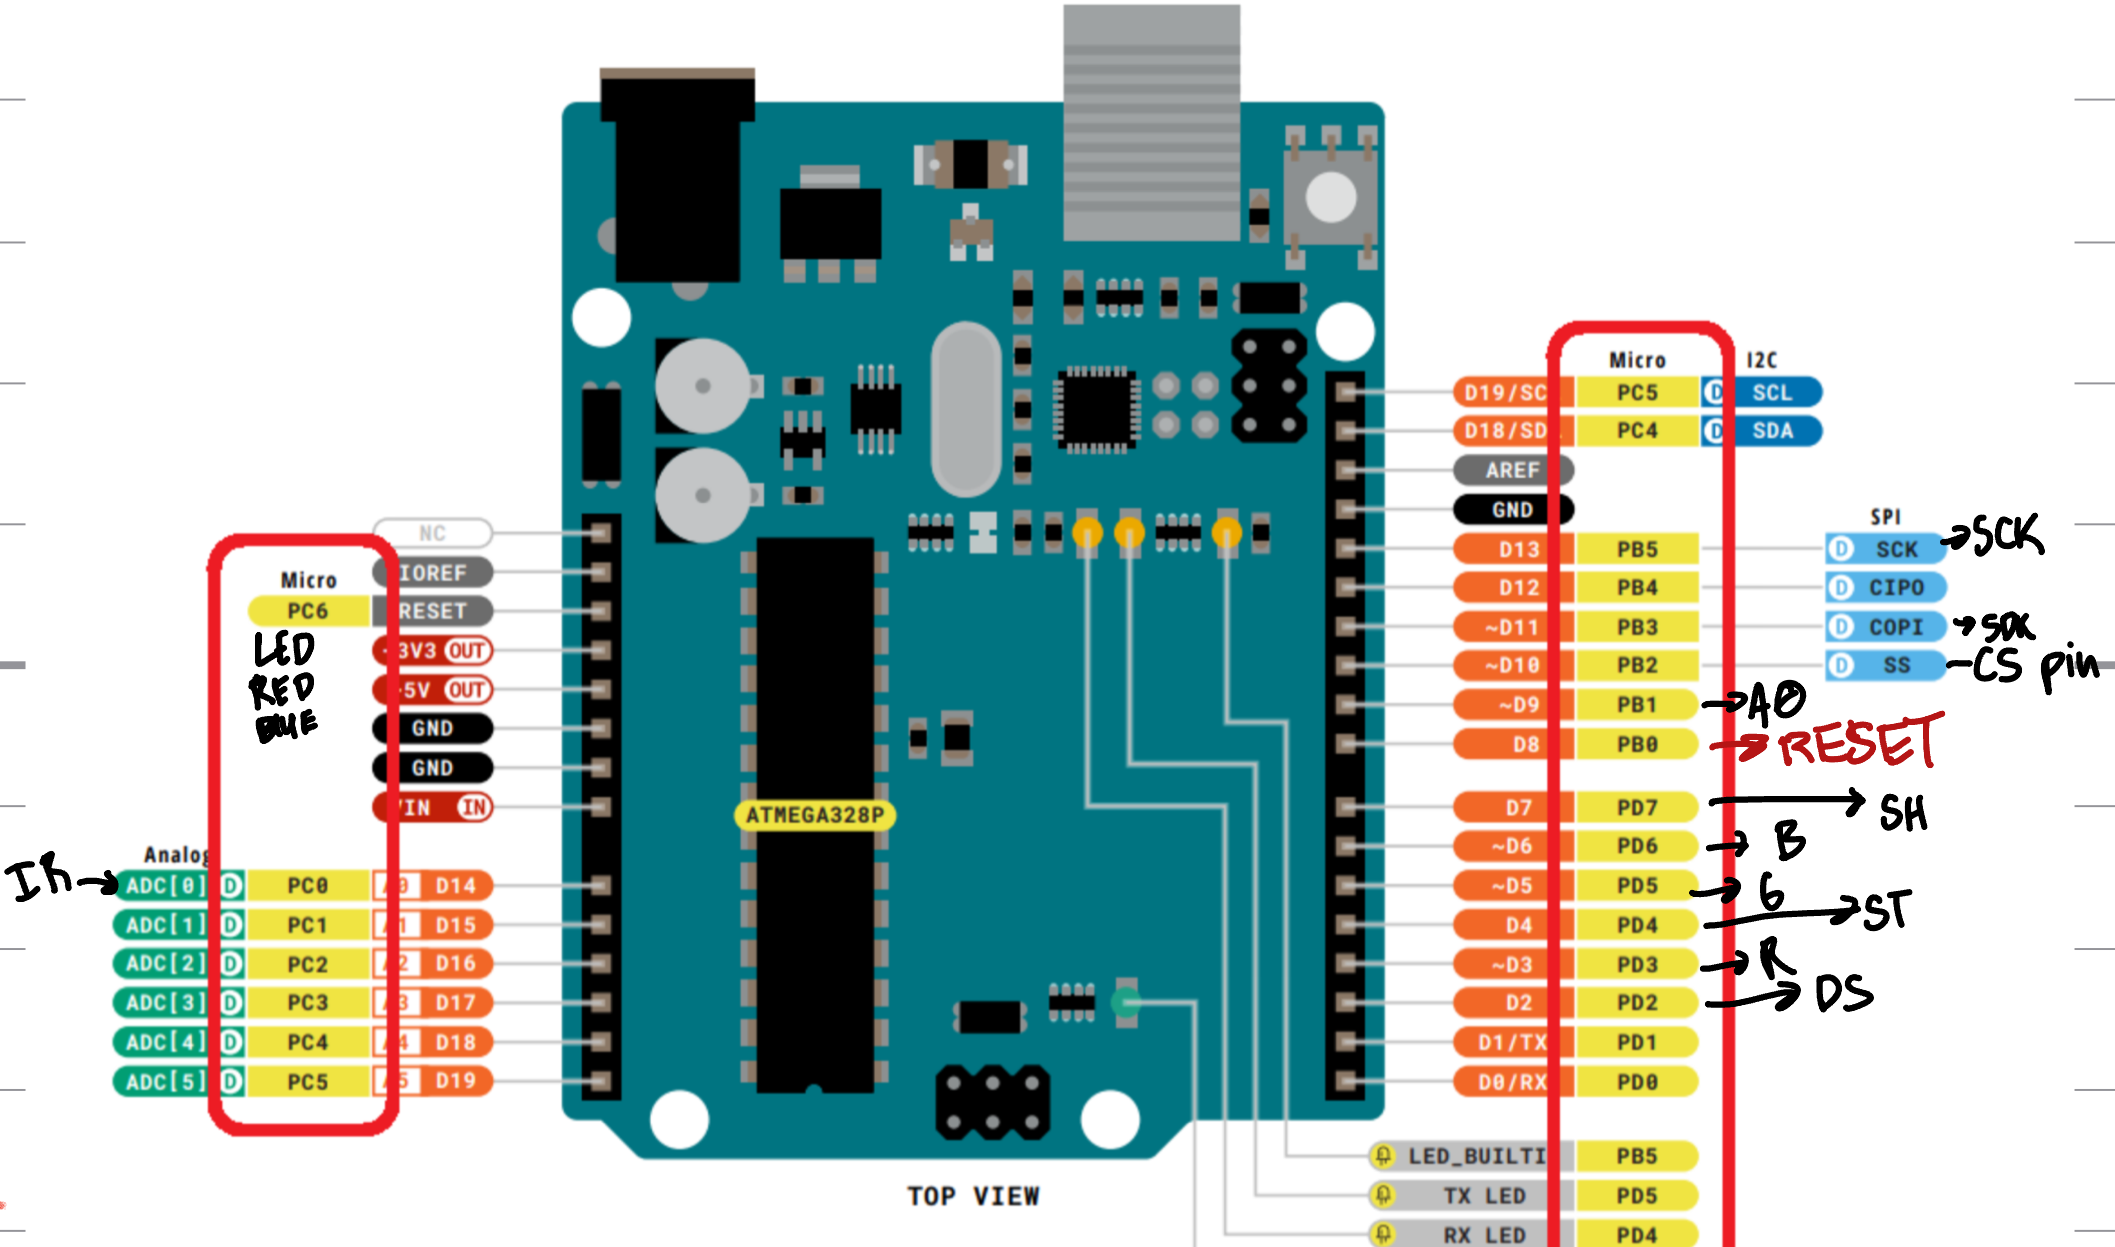
\includegraphics[width=\textwidth]{arduinoDiagram.png}
    % Add arrows or labels using external tools or include the annotated image.
\end{minipage}


\subsection*{Shift Register - 74HC595:}
\begin{minipage}{0.6\textwidth}
\begin{tabular}{ l l l }
   \textbf{1 - Q1}: & Green LED & \quad  \\
   \textbf{2 - Q2}: & Blue LED & \quad  \\
   \textbf{8 - GND}: & GND & \quad  \\
   \textbf{11 - SH CP}: & PD7 & \quad  \\
   \textbf{12 - ST CP}: & PD4 & \quad  \\
   \textbf{13 - OE}: & GND & \quad  \\
   \textbf{14 - DS}: & PD2 & \quad  \\
   \textbf{15 - Q0}: & Red LED & \quad  \\
   \textbf{16 - VCC}: & 5V Power Rail & \quad  \\
\end{tabular}
\end{minipage}%
\hfill
\begin{minipage}{0.45\textwidth}
    \centering
    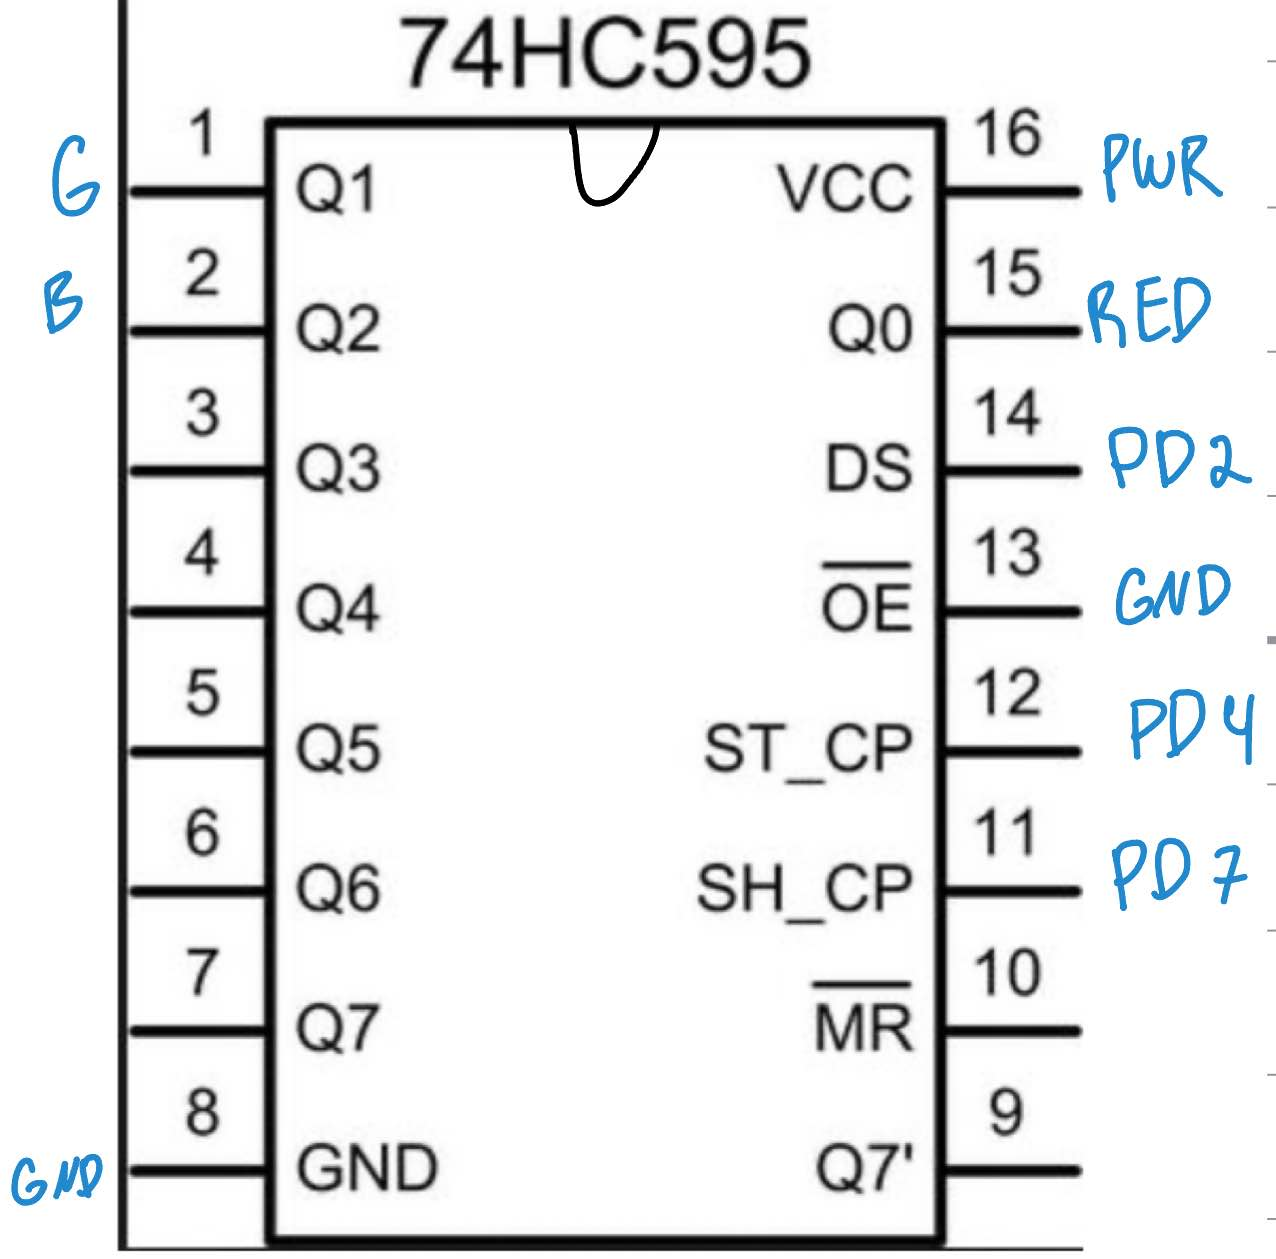
\includegraphics[width=\textwidth]{Shift.jpg}
    % Add arrows or labels using external tools or include the annotated image.
\end{minipage}
\subsection*{Picture of the Circuit:}
    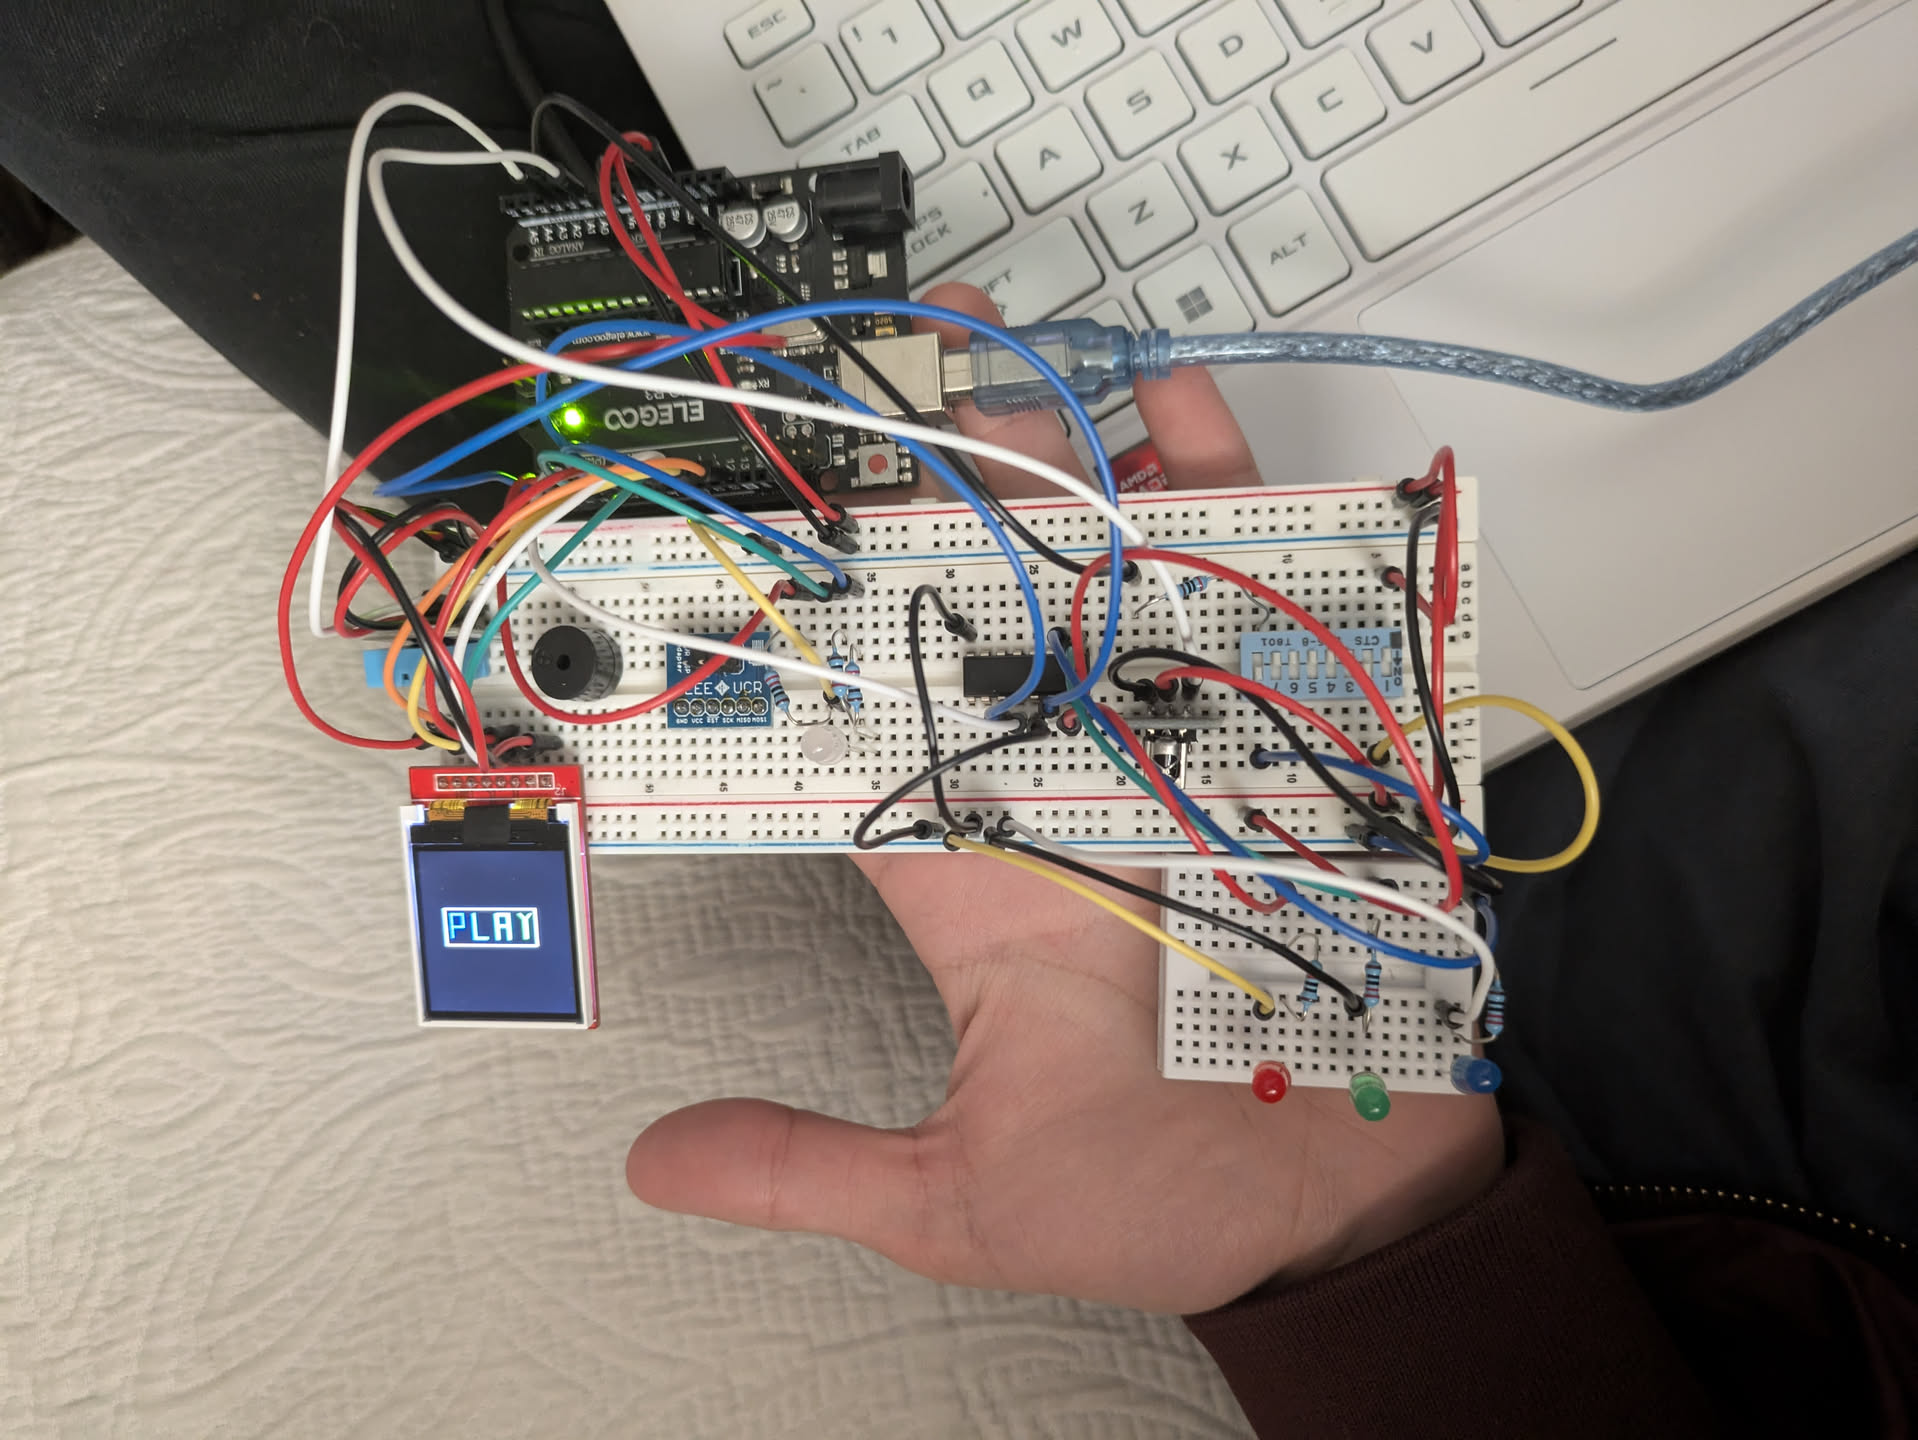
\includegraphics[width=\textwidth]{CircuitPic.jpeg}

\subsection*{Diagram of the Circuit:}
    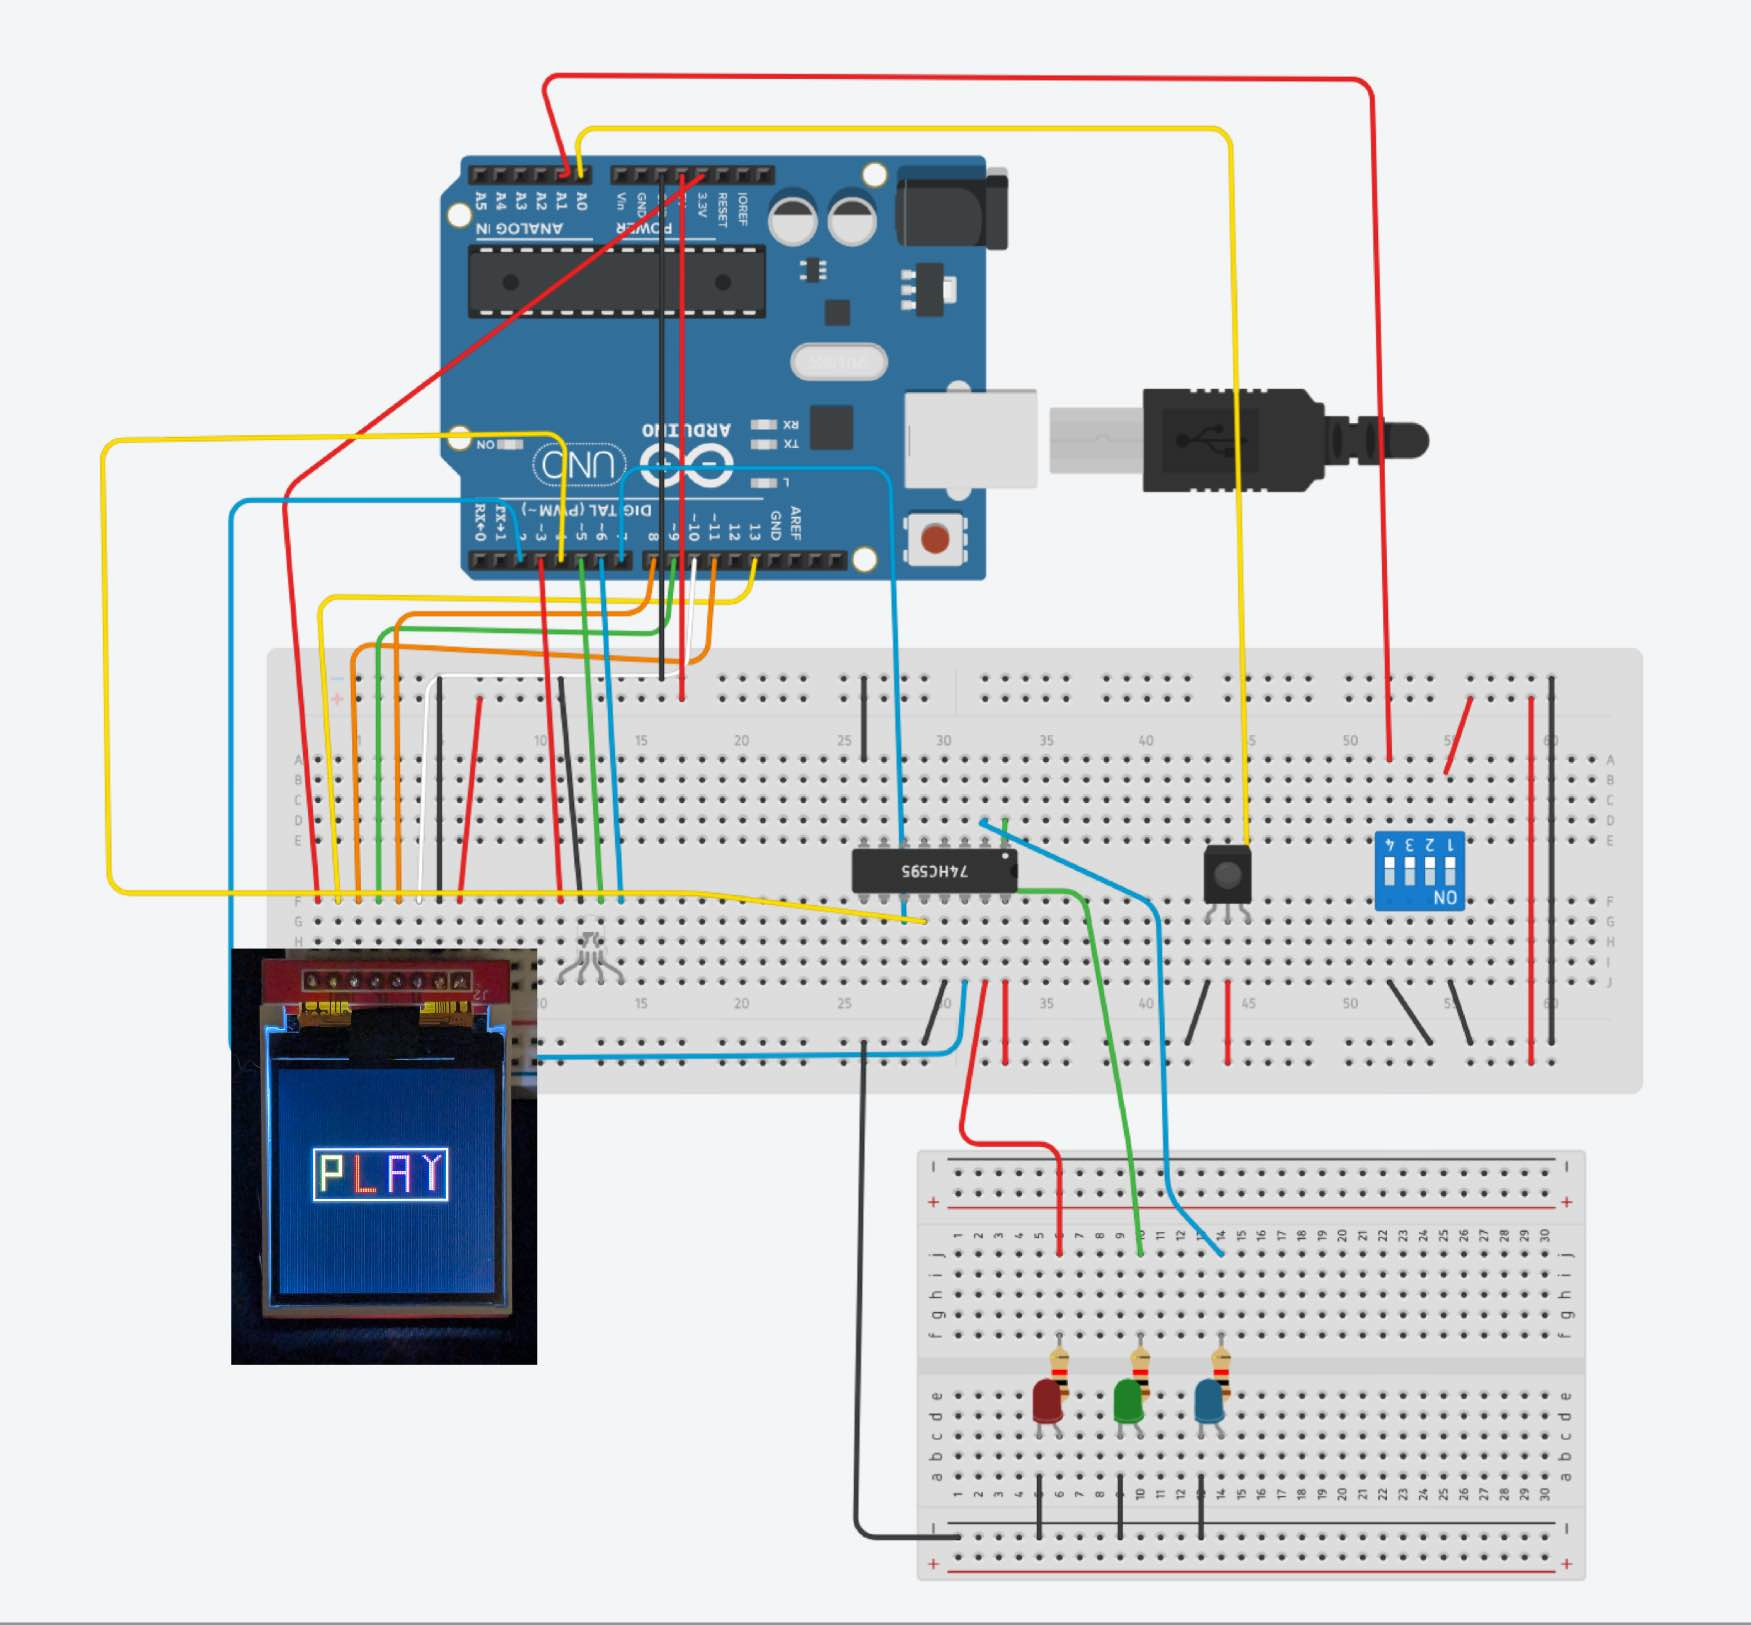
\includegraphics[width=\textwidth]{CircuitDiagram.jpg}

\pagebreak
\section{Tasks Diagram:}
\begin{enumerate}
  \item\textbf{RGB TICK:}
    This is the duty cycle for the RGB LEDs PWM tasks.
    It handles when it is appropriate to have the LEDs on or off.
  \item\textbf{DISPLAY TICK:}
    Helps take care of the two states, the start menu and the active playing menu.
    When you beat the game, it will strobe rainbow through the time that it took you to solve the color.
    Along with the start menu, and the strobing rainbow.
    To strobe the rainbow, I have an array with the colors of the rainbow,
    and I iterate through them.
  \item\textbf{IR TICK:}
    This function is always reading the IR sensor.
    The power button starts the game from the start screen, and from the play state, it rolls a new color.
    While it rolls a new color, it resets the time, currVal, and goes to RGB Tick to ask for a new color.
    Since it grabs the inputs, it updates the currVal when ever it is modified either up or down;
    along with handling overflow.
  \item\textbf{RED TICK:}
    For context, I had issues with digital PWM, and this was my next best option that worked perfectly fine.
    I was able to get this working within the first week and get this out of the way.
    The PWM tick function for the green part of the RGB LED.
  \item\textbf{GREEN TICK:}
    The PWM tick function for the green part of the RGB LED.
  \item\textbf{BLUE TICK:}
    The PWM tick function for the blue part of the RGB LED.
  \item\textbf{SHIFT Tick:}
    This runs in a single state to put the value \textbf{progress} into
    the shiftOut() function. The LEDs are only ever turned on when
    currVal is equal to the target value in the respect hex bits of Red, Green, and Blue.
  \item\textbf{ELAPSED Tick:}
    Tracks the elapsed time in a single state.
    It pauses the elapsed time when you beat the game.
\end{enumerate}

\subsection*{Task Diagram:}
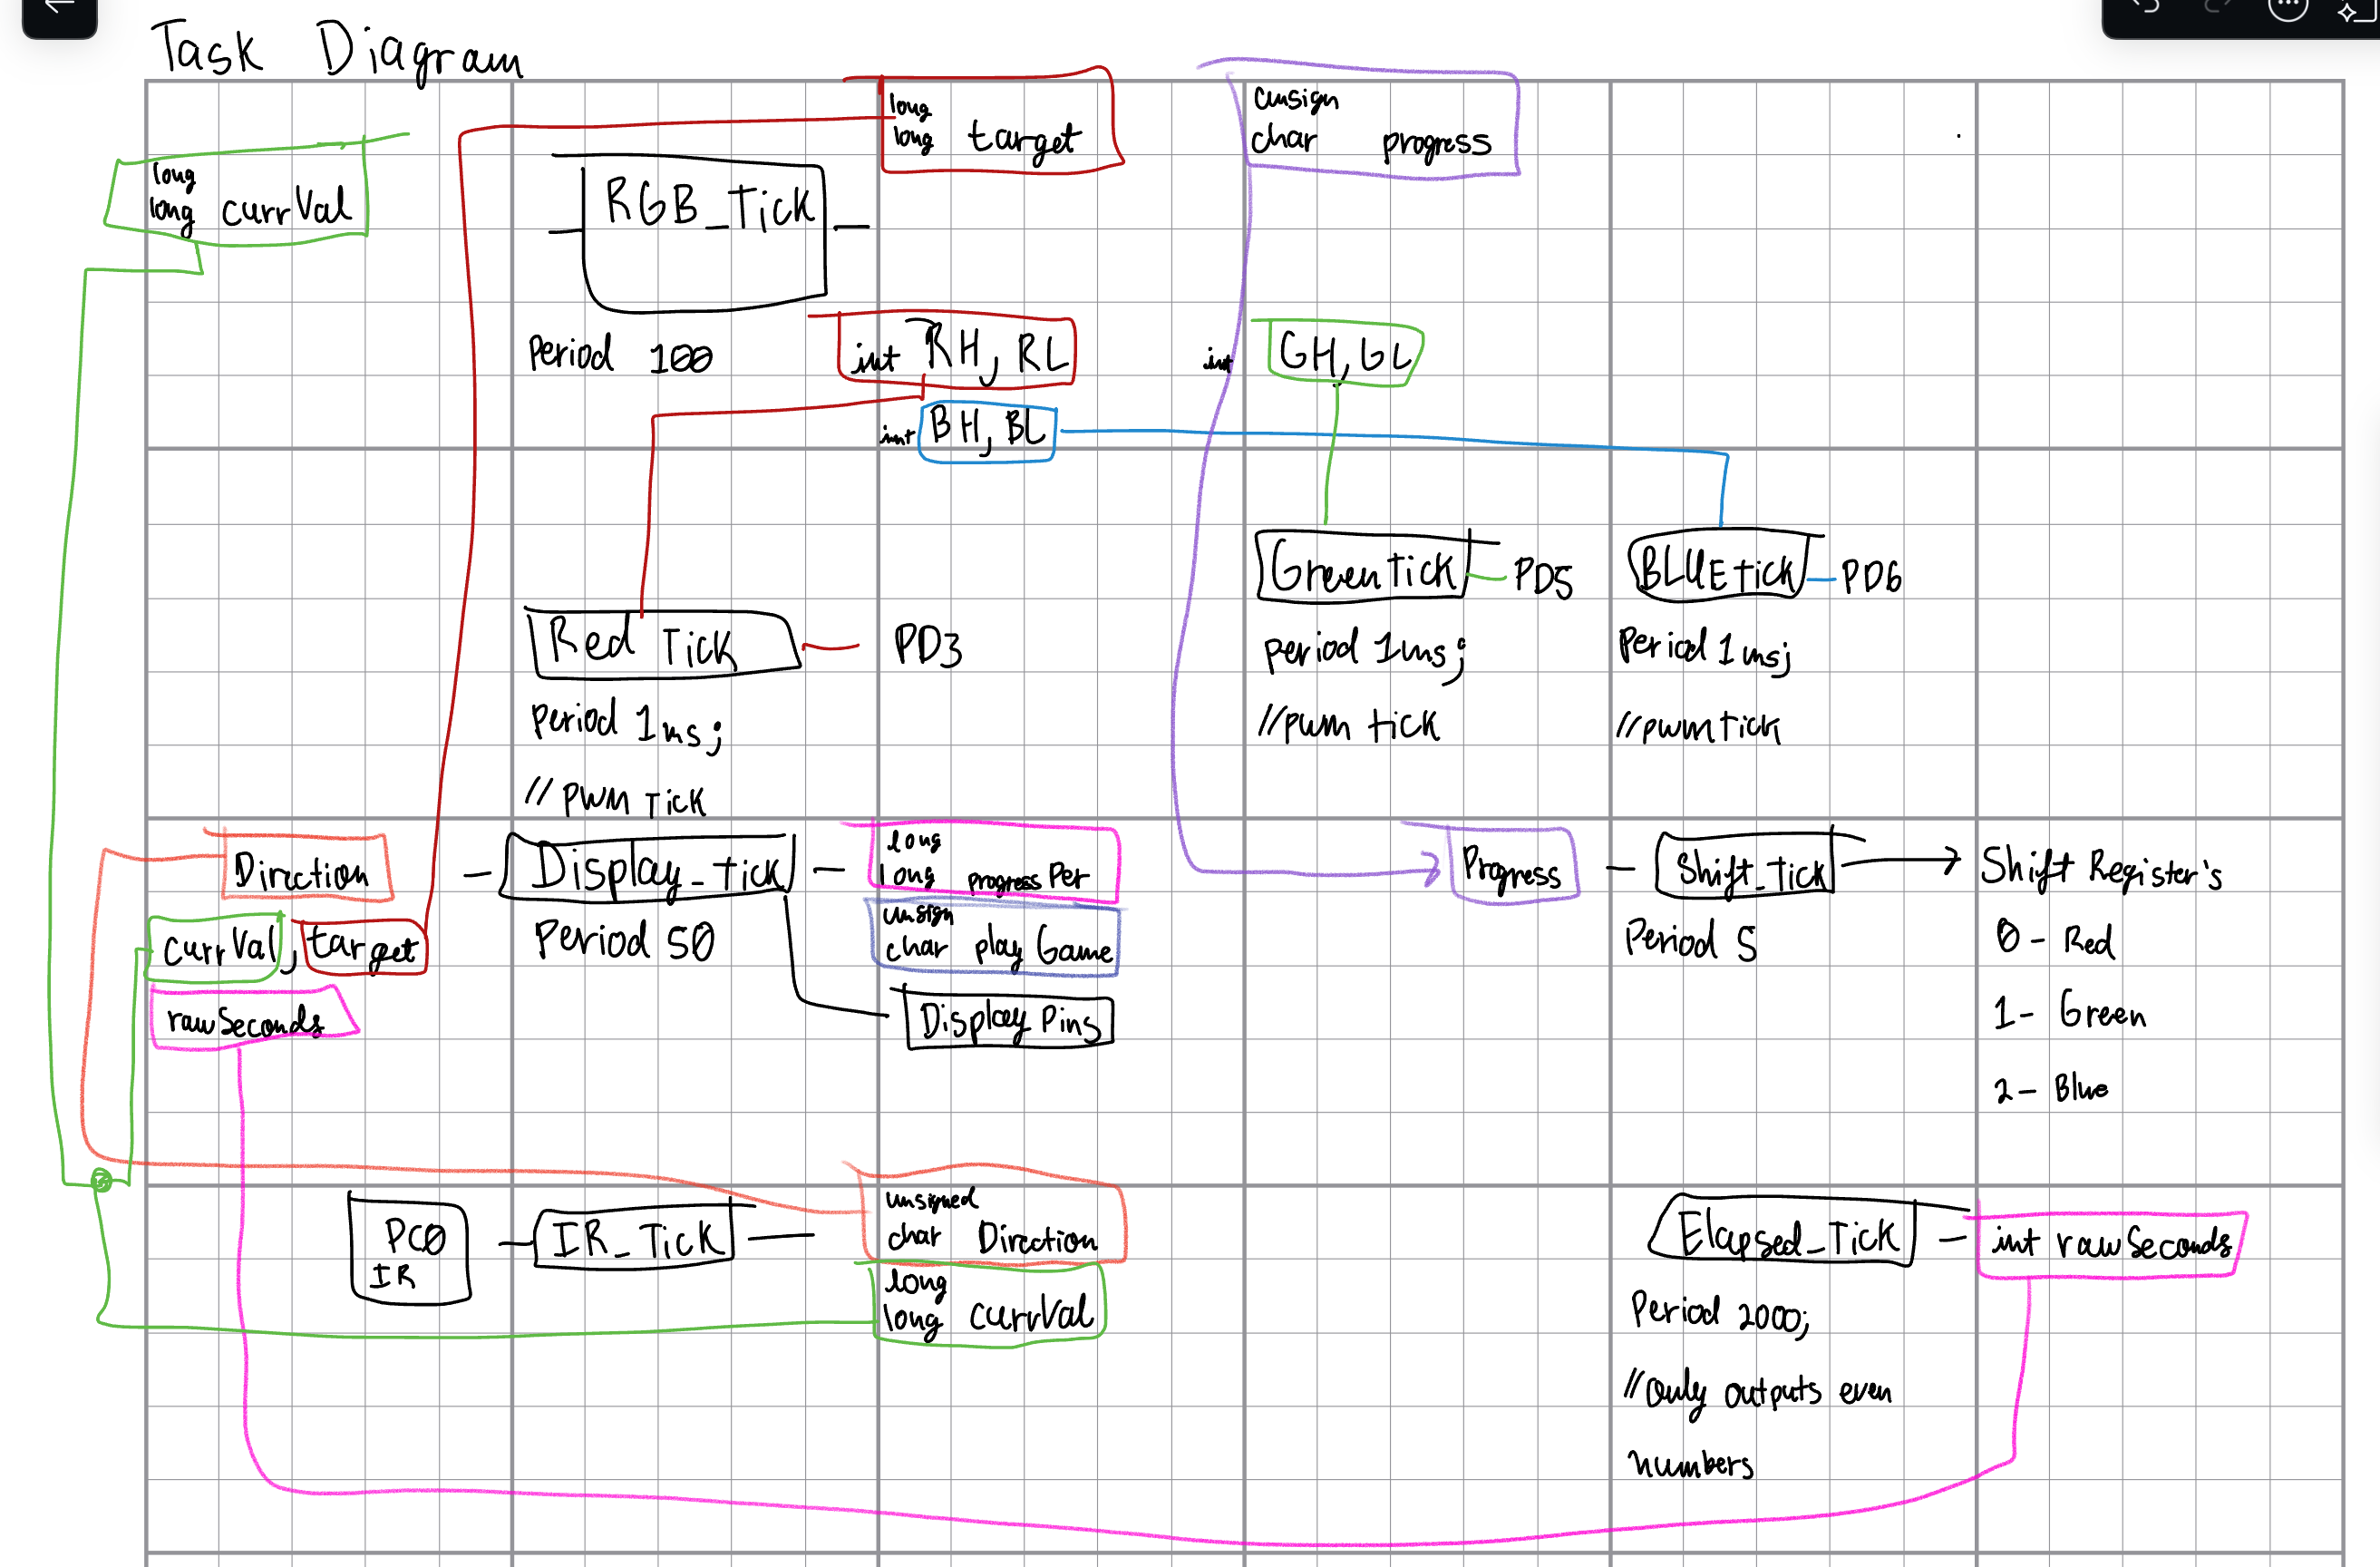
\includegraphics[width=\textwidth]{taskDiagram.png}

\pagebreak

\section{SynchSM Diagrams:}
    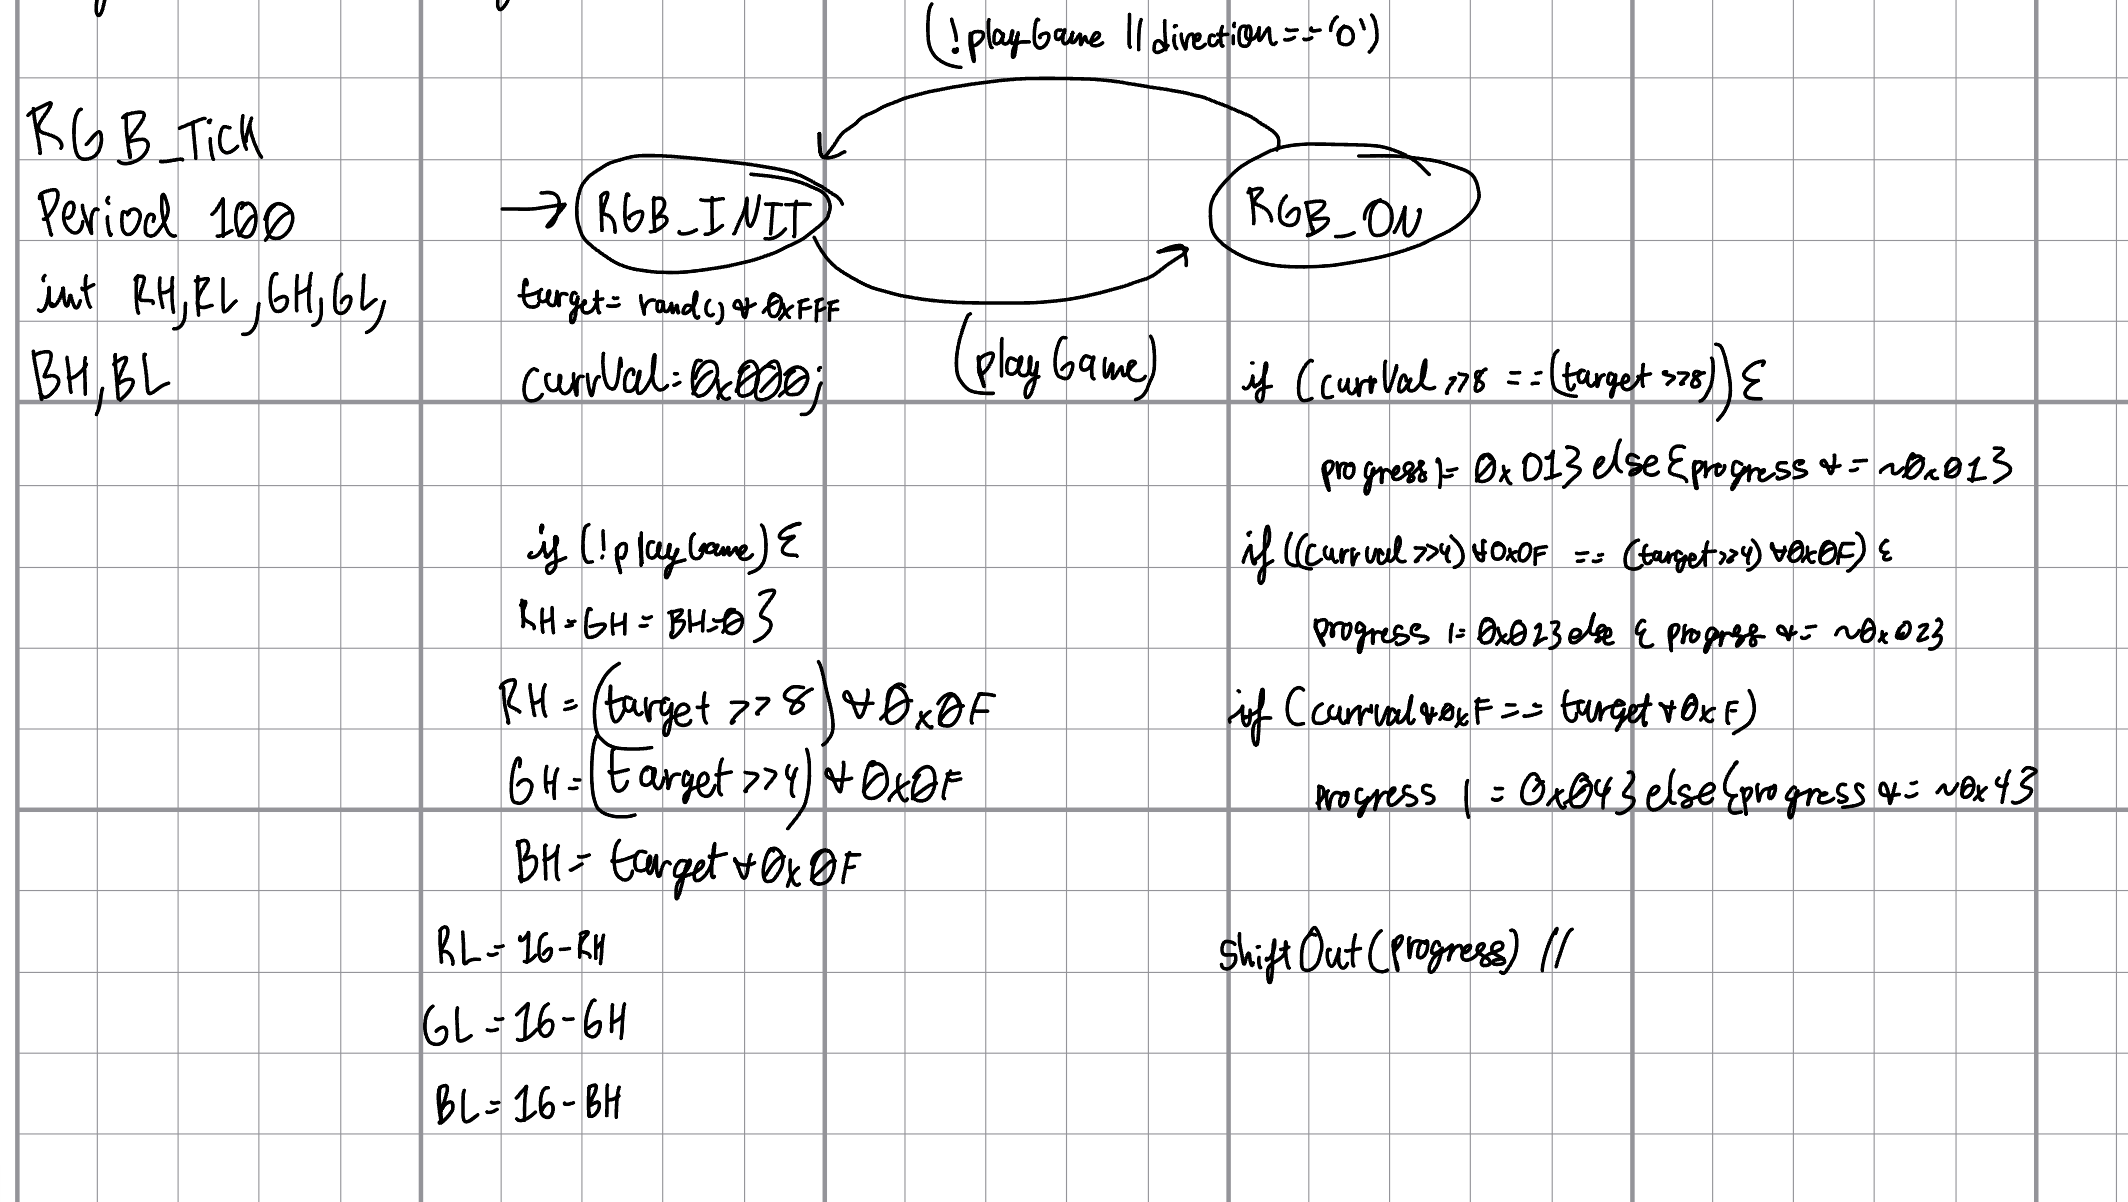
\includegraphics[width=\textwidth]{RGBTick.png}
    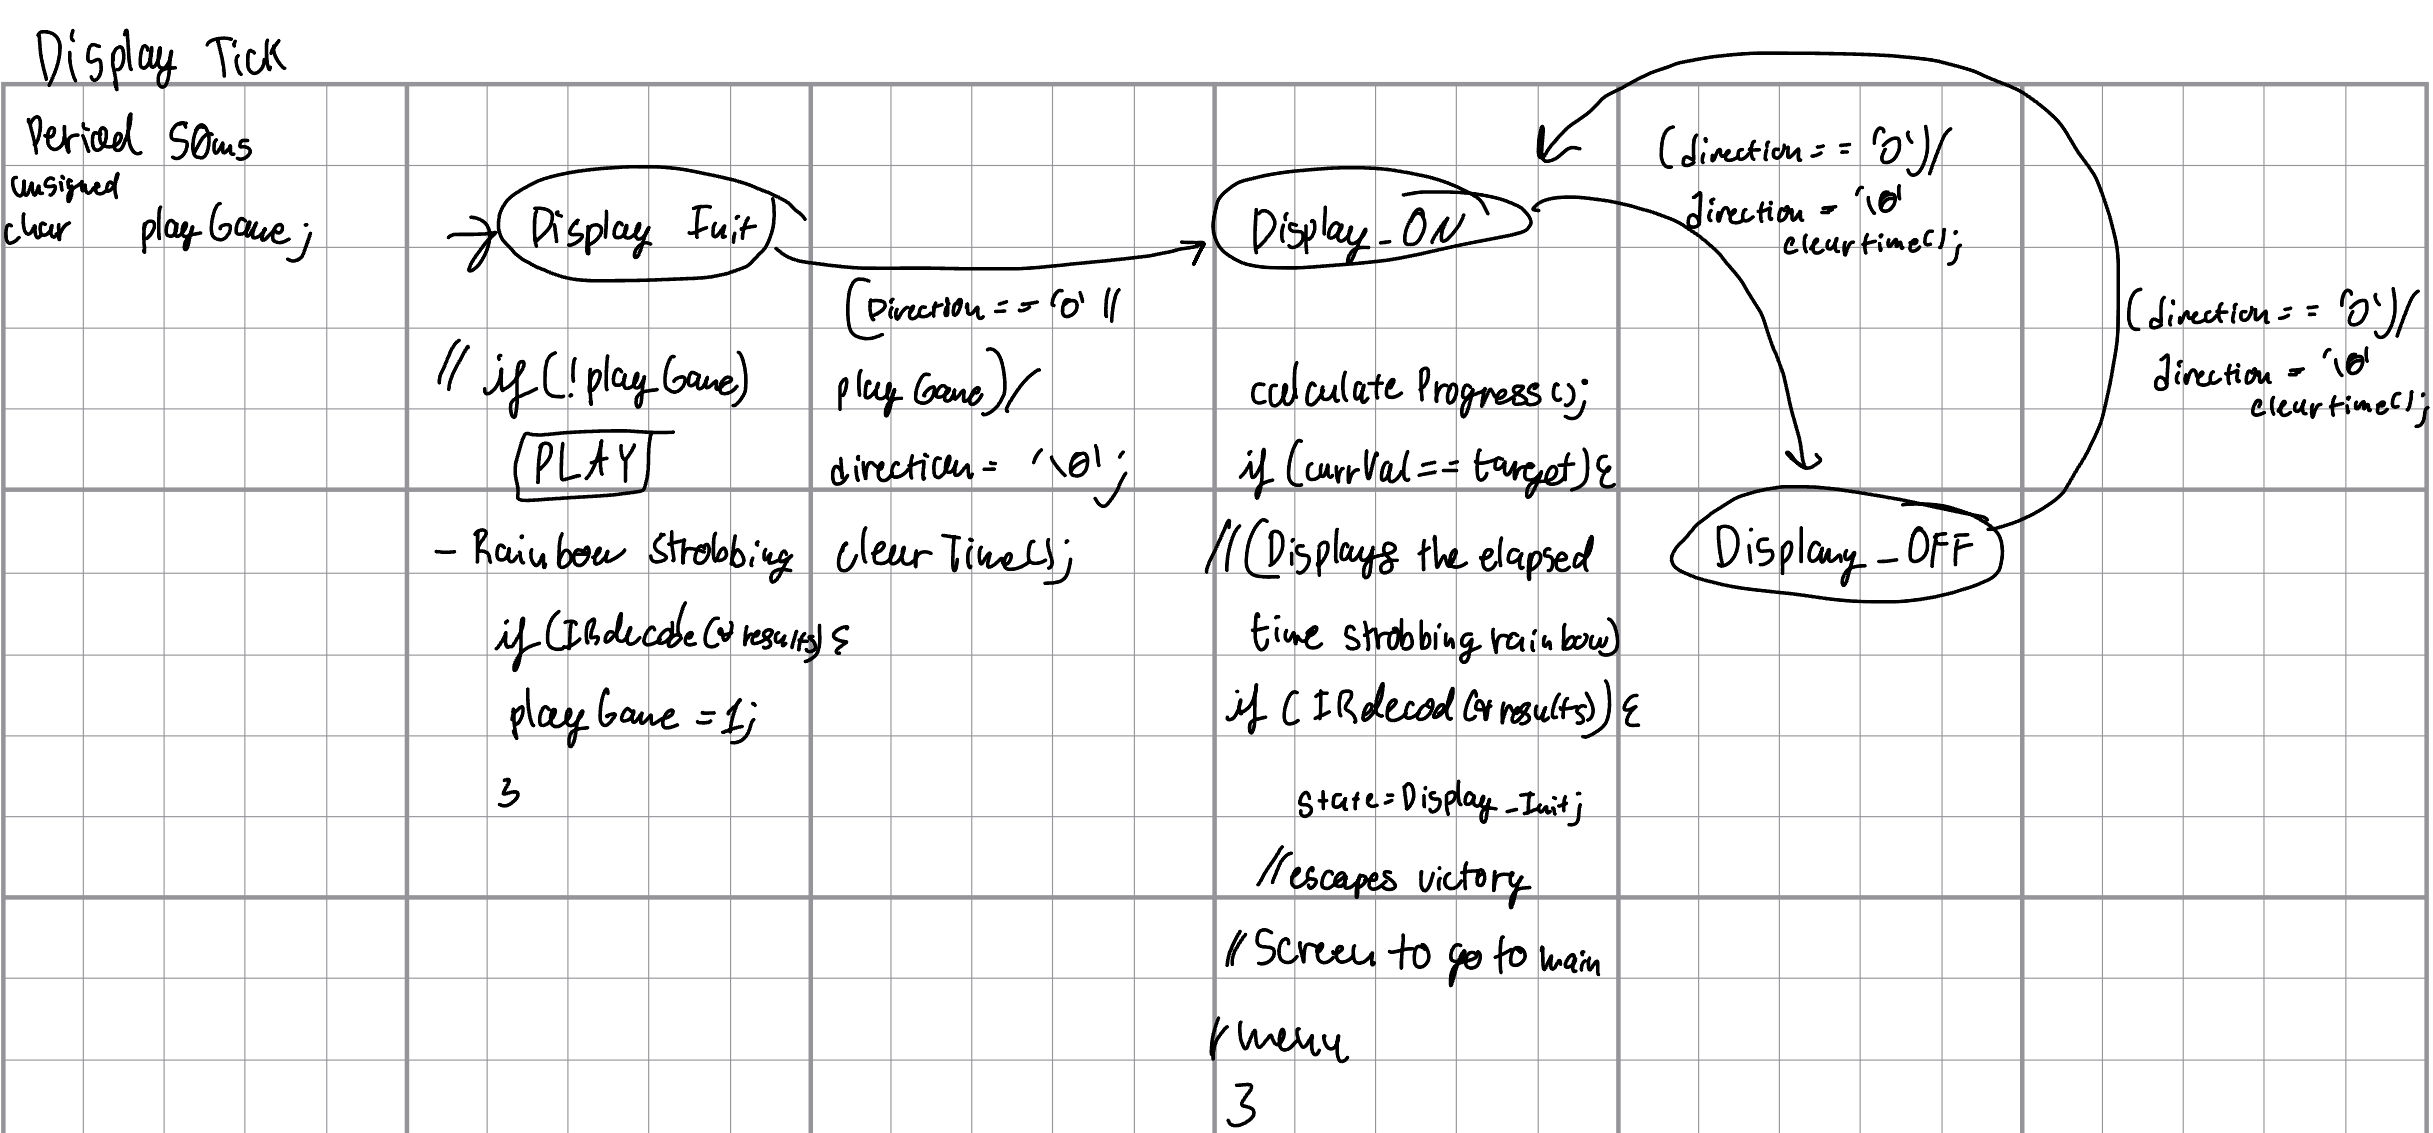
\includegraphics[width=\textwidth]{DisplayTick.png}
    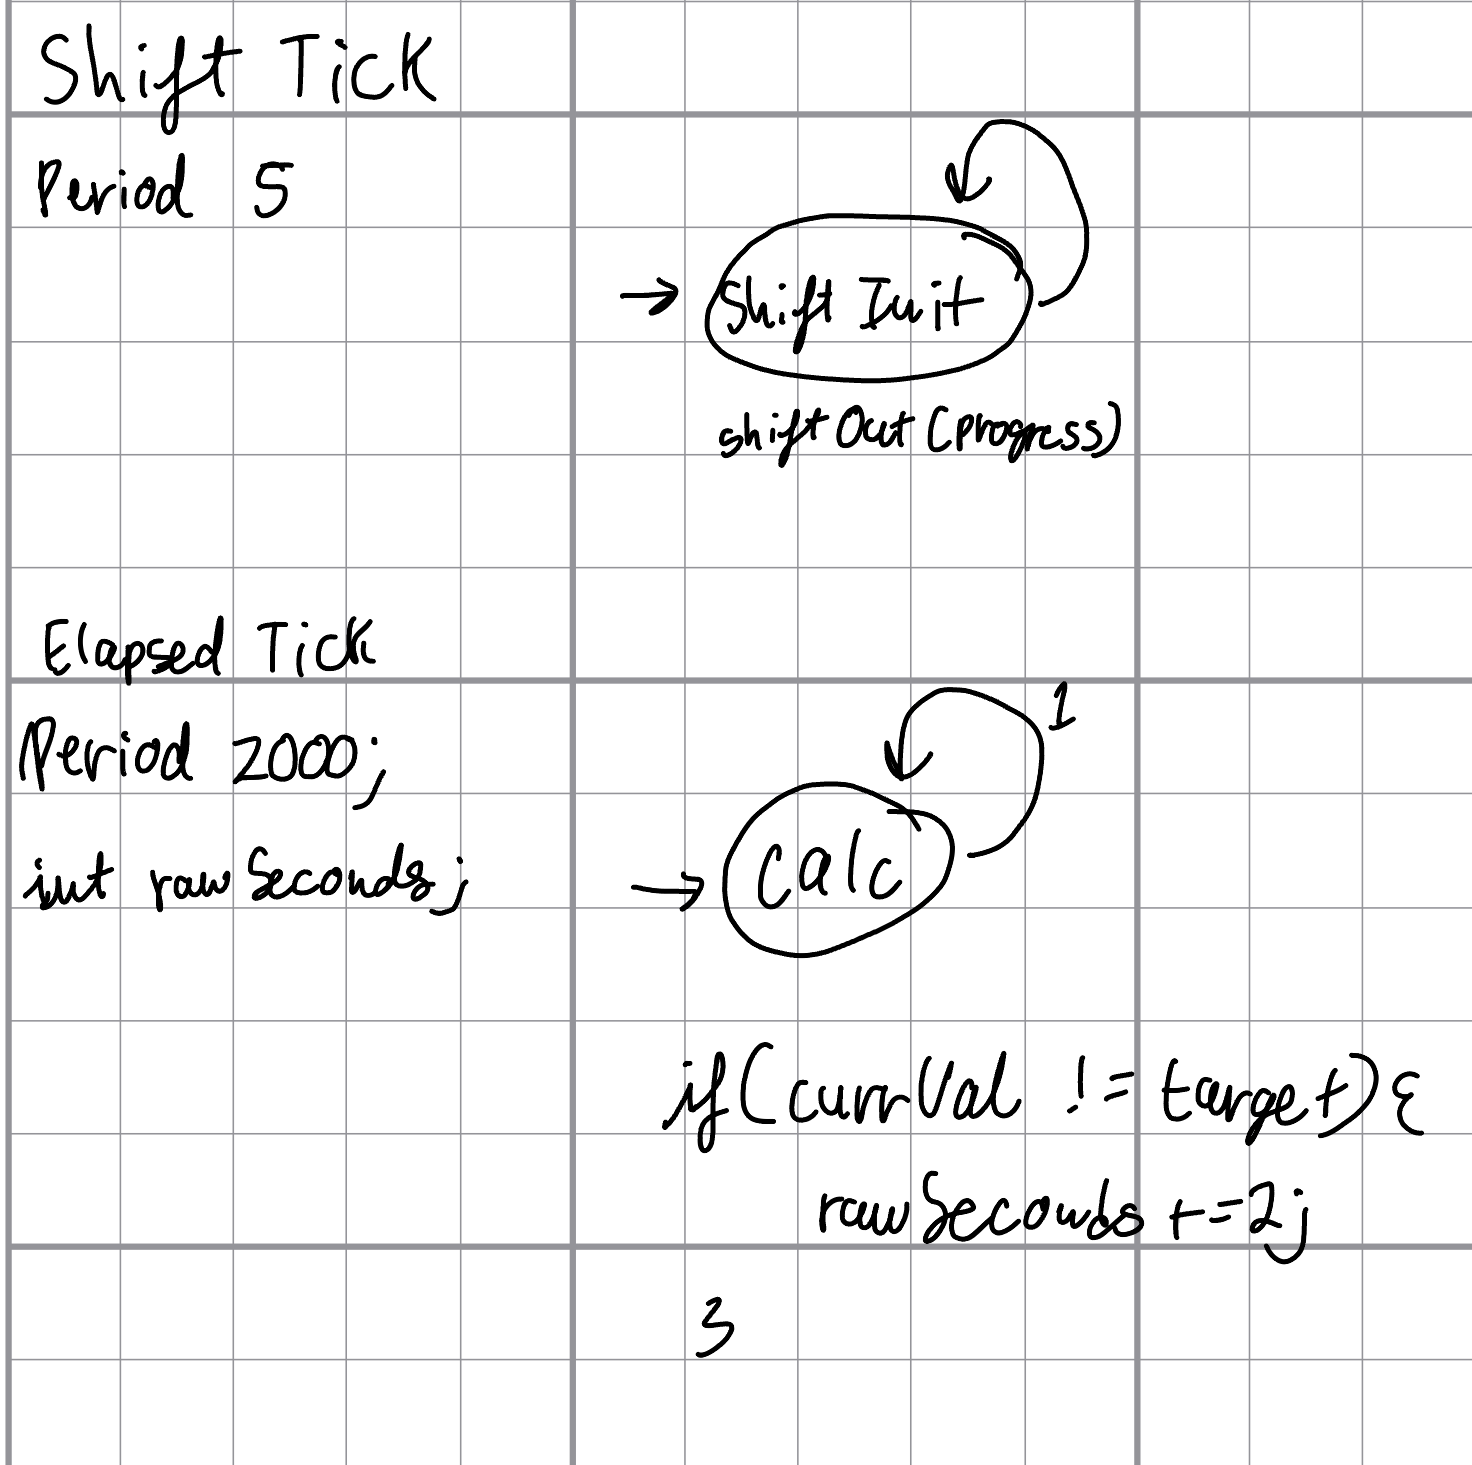
\includegraphics[width=\textwidth]{ShiftTick.png}

\pagebreak
    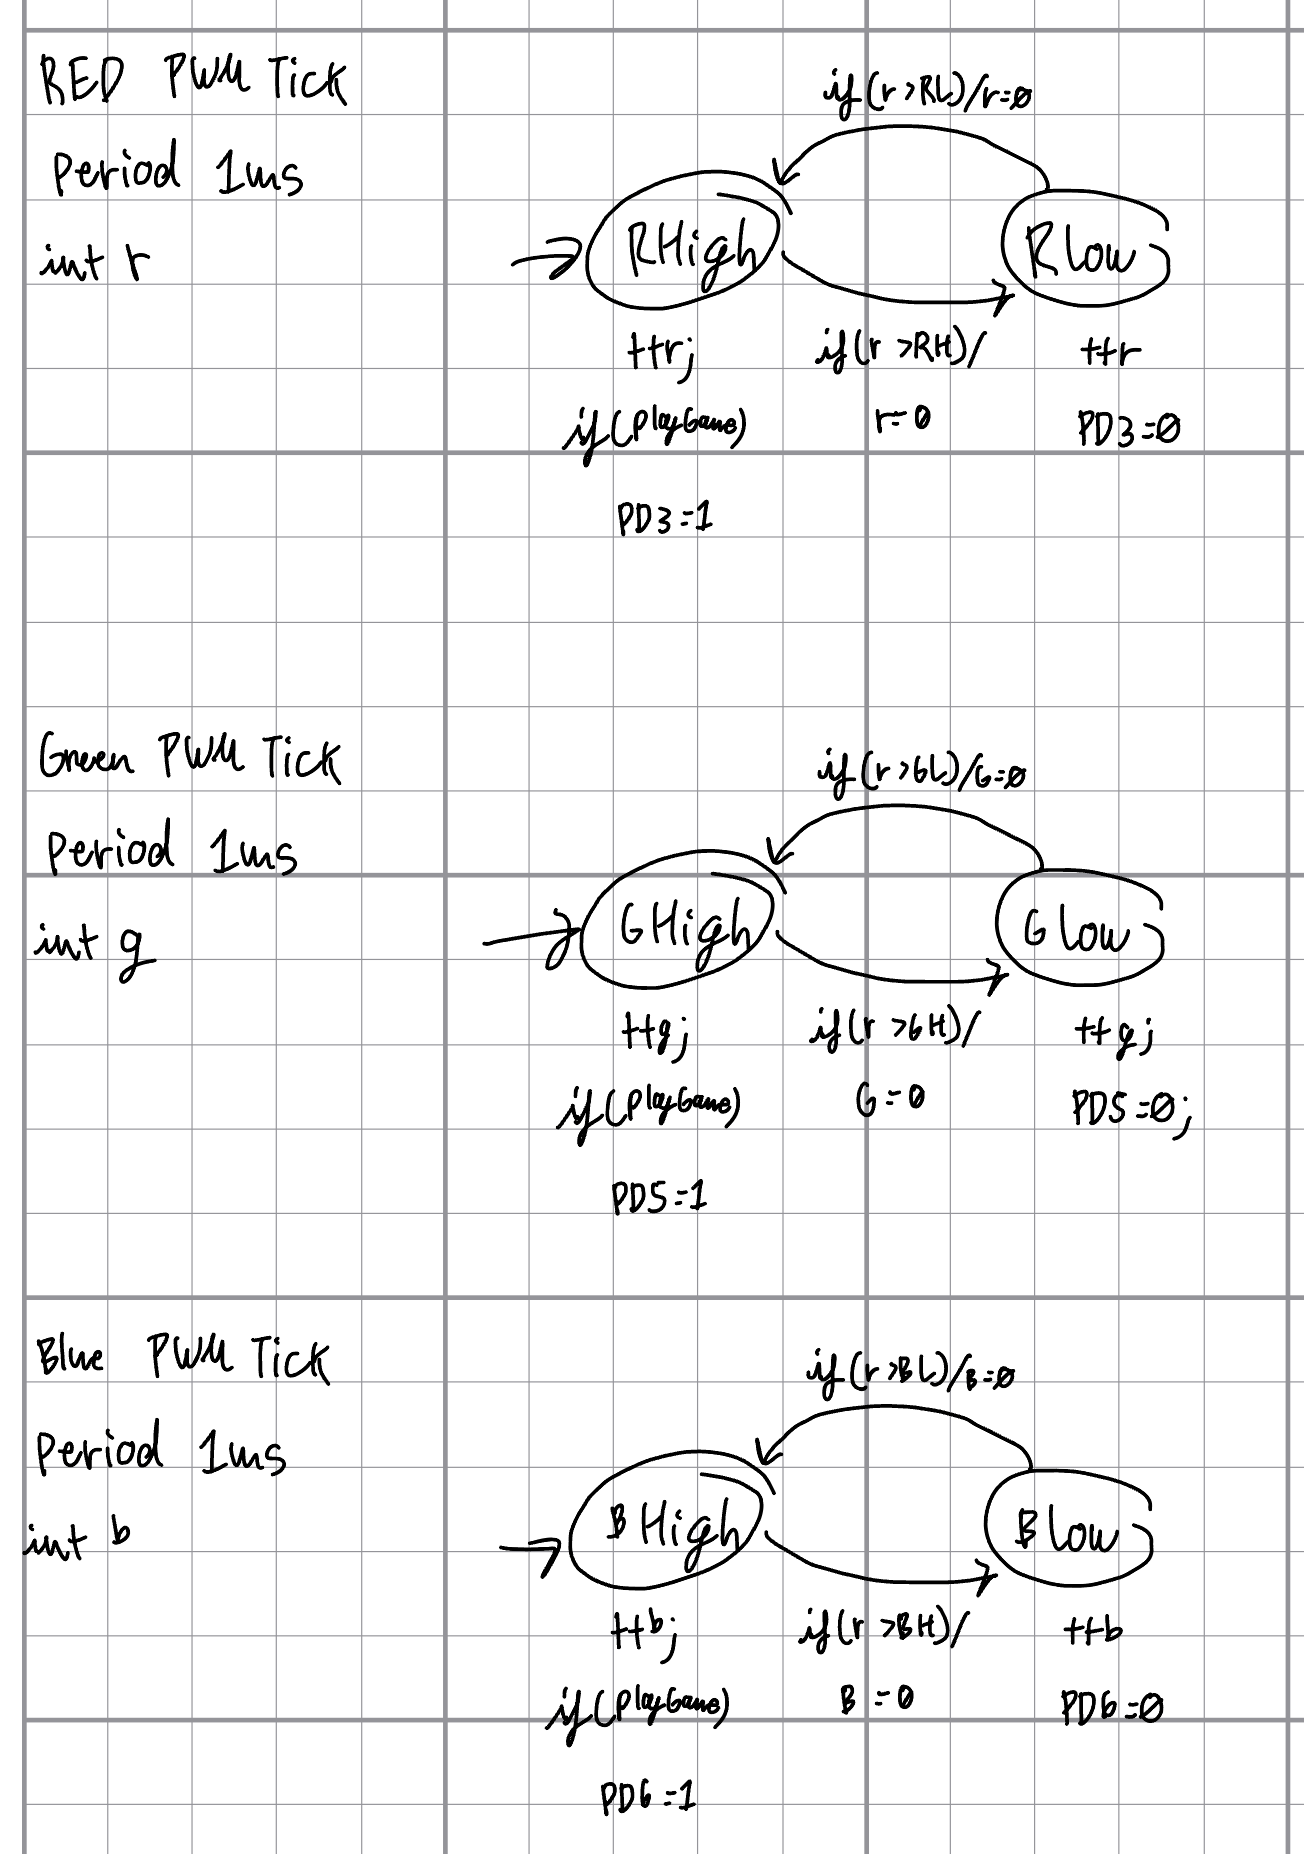
\includegraphics[width=0.9\textwidth]{PWMTicks.png}

\pagebreak
As a side note, after every single button press, the screen gets updated.
For example after all the number buttons, the command updateHex() runs.
This command serves to update the screen as the hex currVal has been updated.

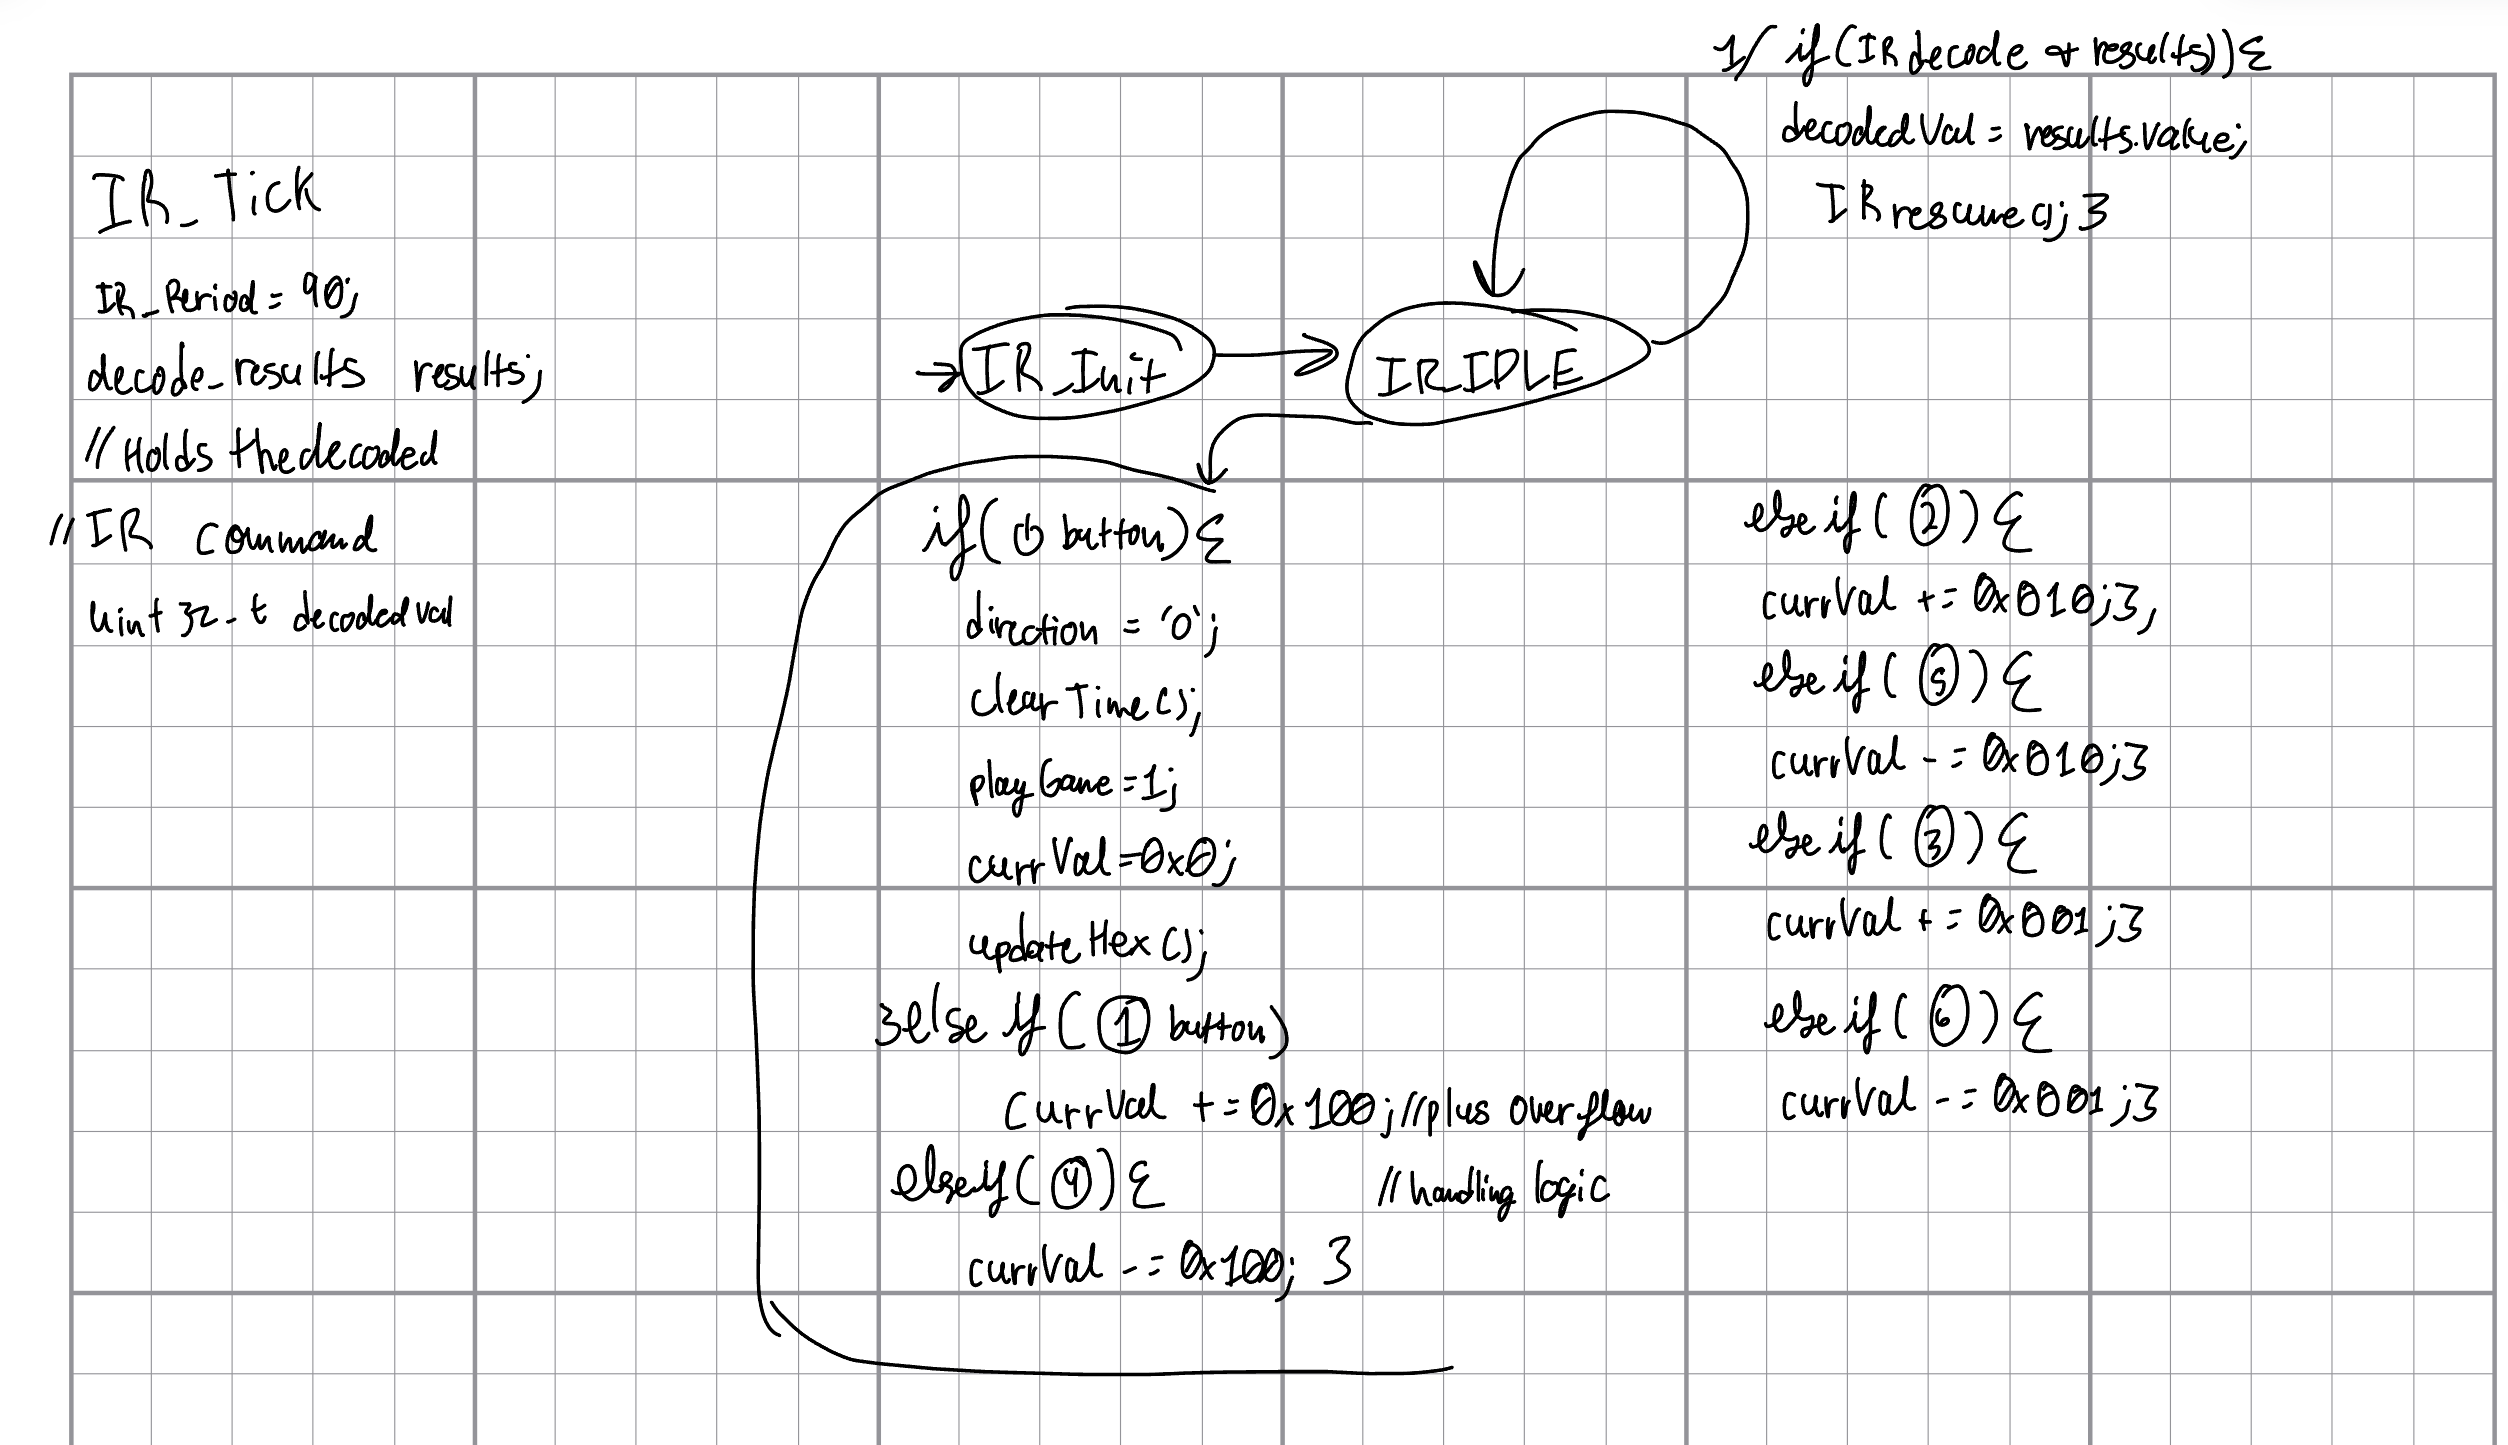
\includegraphics[width=1.2\textwidth]{IRTick.png}


% --------------------------------------------------------------
%     You don't have to mess with anything below this line.
% --------------------------------------------------------------

\end{document}t
